% =========================================================================
\chapter{Introduction}
\label{ch:intro}
% =========================================================================

\claim{A self-evolving harness stalls not for lack of intelligence but for
lack of a readout: we demonstrate that its evidence is false, replace that
evidence with a graph-native record, retype its candidate surface, find
that outcomes do not separate in either direction at the resolution this
bed affords --- measured on three seeds per arm --- and locate the missing
organ, ``did that edit work?'', which no system in the field measures.}

% -------------------------------------------------------------------------
\section{The system under study}
\label{sec:motivation}
% -------------------------------------------------------------------------

An agent is a model plus a harness, and the harness is frequently the
dominant performance lever. That makes the harness a natural target for
automatic optimization, and a literature of self-evolving agents has grown
around the idea~\cite{survey-selfevolve}. Most of it evolves prompts,
workflows or agent code. Very few systems close the loop at the level of
the harness itself.

HarnessX/AEGIS~\cite{aegis} is one of the few, and it is the system this
thesis takes as its object. Its loop runs in six stages. Each round the
solver attempts the bed under a fixed configuration. A \textbf{Digester}
reads every trajectory --- failures and successes alike; the success
template instructs it ``not to celebrate'' but to name the reusable
strategy and any latent fragility --- and writes a per-task dossier. A
\textbf{Planner} synthesizes the dossiers into one landscape. An
\textbf{Evolver} authors zero or more candidate edits to the harness's
configuration, tools, prompt or processors, each as a manifest plus an
applied configuration. A \textbf{Critic} judges each candidate, may
interrogate the Evolver, and audits the candidates as a set against the
scoreboard. Survivors face five deterministic gates, cheapest first: a
\emph{structure} gate enforcing twelve evidence invariants (every cited
anchor must exist on disk and point inside its trajectory); a
\emph{novelty} gate against a ledger of refuted candidate signatures;
canonicalization; a \emph{counterfactual} gate that replays the proposed
processor chain over the previous round's passing tasks and rejects on any
change to output or exit reason; and a synthetic-task \emph{replay} smoke.
Every role runs behind read and write scope gates that forbid it the
harness source and the histories of other runs. The loop invokes itself
selectively, on an actionability score, and shipped candidates are scored
afterwards on the tasks they predicted they would flip.
Figure~\ref{fig:official} is the system's own picture of itself;
Figure~\ref{fig:loop} opens its \emph{adapt} vertex into the six stages
just described and marks the seams at which Chapter~\ref{ch:ghx}
attaches.

\begin{figure}[t]
\centering
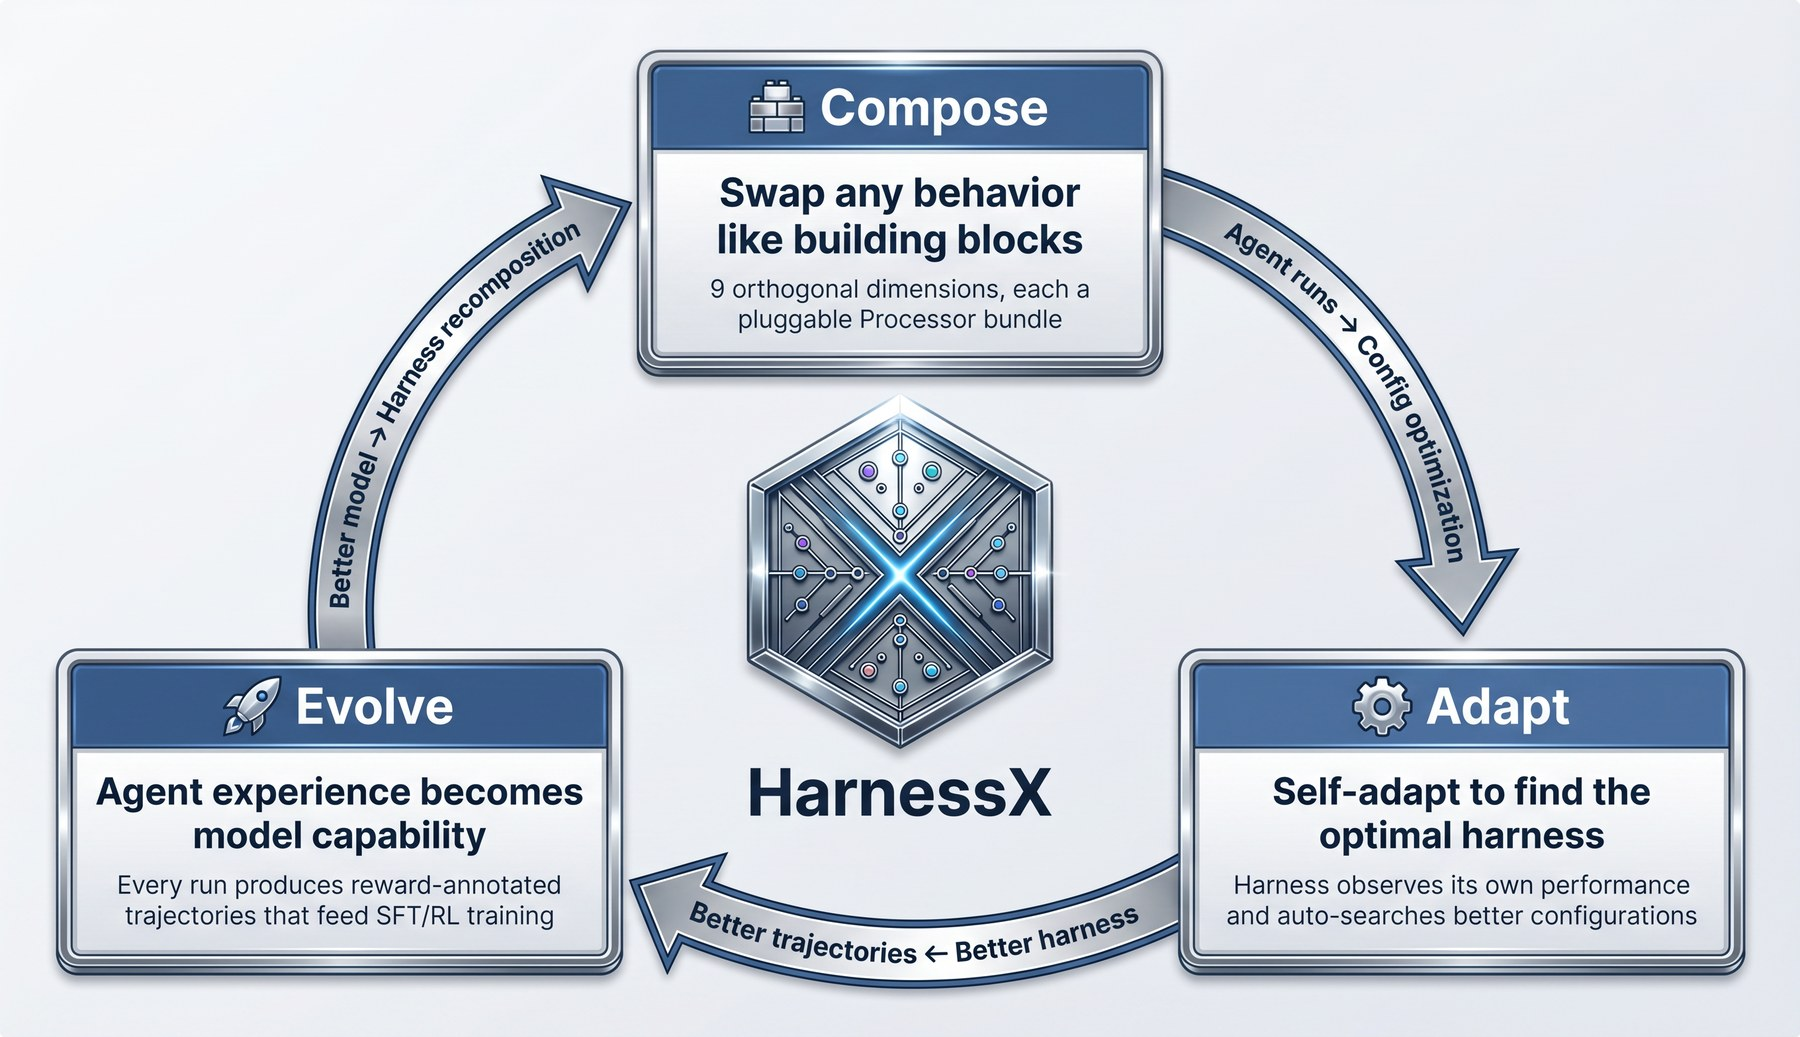
\includegraphics[width=0.88\textwidth]{fig/harnessx_architecture.jpg}
\caption[The official HarnessX overview]{The official system's own
overview of itself: \emph{compose} a harness from pluggable processor
bundles, \emph{adapt} it by letting it observe its own performance and
search better configurations, \emph{evolve} models on the trajectories
it produces. Reproduced from the HarnessX repository's documentation
assets~\cite{aegis}. The loop this thesis executes is the \emph{adapt}
vertex.}
\label{fig:official}
\end{figure}

This is more governance than any neighbouring system carries
(Chapter~\ref{ch:related}), and it is why the system was chosen: a loop
this well-guarded is the right one on which to ask what the guards can and
cannot see.

\subsection*{What we met when we tried to reproduce it}

The paper's GAIA headline is a $+13.6$-point gain that appears only once
variants are isolated inside an ensemble~\cite{aegis}. Reproducing it ran
into the release. The variant pool and
ensemble routing that headline rests on are absent from the released code,
which is a single lineage with a \texttt{ship\,|\,no\_op} decision. The
released GAIA runner defaults to a single task, ships no launch script and
no committed numbers, and the fourteen-round GAIA-64 pilot the authors'
own narrative describes has its results directory excluded by
\texttt{.gitignore}. The one complete experiment in the repository is on a
different benchmark entirely \F{19}. Three further specifications in the
paper are not in the code: the global ratchet forbidding any solved task to
be given back, the $\pm 5\%$ noise threshold on retention, and three seeds
per cell.

\emph{So there is a number, and there is no recomputable number.} What we
ran is the released system --- not the system the paper describes --- and
this distinction is maintained throughout. Every divergence between the two
is recorded in Appendix~\ref{app:deviations}.

% -------------------------------------------------------------------------
\section{What was run, and why this bed}
\label{sec:what-was-run}
% -------------------------------------------------------------------------

The system was vendored byte-for-byte under a sha256 manifest enforced by
tests, and executed at scale: six claim-bearing campaigns on the
\textbf{100-task no-pixel bed} drawn from GAIA's text-only split ---
one bed for every number in this thesis (\S\ref{sec:beds}).
Each campaign is read over its formal sixteen-round window, so
\textbf{96 rounds and 8{,}393 fresh task evaluations} enter the evidence
base \F{51}. To our knowledge this is the system's first independent execution.

\subsection*{Why GAIA, and why these hundred tasks}

Four reasons, in the order they weighed.

\begin{enumerate}
  \item \textbf{It is the authors' bed.} The paper's headline is a GAIA
        number and its own narrative describes a GAIA pilot, so a GAIA bed
        is the one on which the released system can be held to its
        paper.
  \item \textbf{The text-only split keeps the solver inside what the
        recorder can attribute.} GAIA's text-only tasks are answered
        through tools the harness owns --- shell, file reads, web search
        --- so every step of a trajectory is an event the execution graph
        of Chapter~\ref{ch:ghx} can record. Three of the split's 103 tasks
        carry pixel content the recorder cannot attribute; they are
        excluded, which leaves 100. Every number in this thesis is on
        those 100 (\S\ref{sec:beds}).
  \item \textbf{There is room.} Across the six campaigns the union of
        tasks ever solved is 97 of the 100, against a best single round of
        76: twenty-one tasks of headroom that the loop's own history shows
        to be reachable, and 47 tasks that pass sometimes but not
        reliably \F{16}. The bed is neither saturated nor floor-bound, so a
        harness effect has somewhere to appear.
  \item \textbf{It is small enough to re-run whole, every round.} A
        hundred tasks can be attempted in full sixteen times per campaign,
        which is what makes same-configuration re-measurement --- the
        instrument Chapter~\ref{ch:design} is built on --- affordable at
        all.
\end{enumerate}

\emph{Claim-bearing subset, stated up front.} Two further graph campaigns
were flown before the graph layer was correct. They are excluded from
every number and every narrative in this thesis, and are named here only
so that the count of campaigns flown is complete. Two executed rounds
also fall outside the formal window and are excluded with it: the baseline campaign's seventeenth
round, which no reported statistic uses, and a one-round aborted first
launch of the graph campaign,
which reached its baseline draw and was restarted. Neither carries a ship,
a candidate, or a uniquely-solved task, so no number in this thesis moves
with them \F{51}. The 8{,}393 figure counts fresh
evaluations only; a different denominator, 9{,}600 task evaluations
including tasks carried through no-op rounds, appears in
Chapter~\ref{ch:design} where per-task census statistics need it. Both are
stated with their scope wherever they are used.

% -------------------------------------------------------------------------
\section{What running the baseline revealed}
\label{sec:baseline-revealed}
% -------------------------------------------------------------------------

The loop's central evidence signal --- whether a tool call's output was
\emph{used} --- is structurally blind, and the blindness follows from its
own construction.

The column grades a call by whether the immediately next assistant message
shares a verbatim substring of at least twenty characters with the tool
output. GAIA final answers have a median length of nine characters. A short
fact cannot clear that floor however it is used \F{3}.

That conclusion needs no experiment: the first premise is a property of
the code and the second a property of the benchmark. What the data add
is reach. The rate at which the column applies its negative verdict to
answer-carrying calls --- $75.0\%$ of 559 such calls \F{2} --- is
reported in \S\ref{sec:evidence-audit} as a property of the column's
output, with the limit that a call on a passing path holding the answer
is not thereby shown to have \emph{caused} the pass.

The verdict is not inert. It reaches $86.0\%$ of dossiers \F{4}, is quoted
verbatim in accepted candidates \F{5}, and one candidate shipped on it
\F{6}.

Everything else about the baseline treads water: a flat plateau, an edit
ledger that fixes one thing and breaks another, and shipped-edit margins
inside the same-config re-measurement envelope.

\medskip
\noindent This produced the thesis's hypothesis.

\begin{quote}
\textbf{H1.} The loop's failure is an \emph{evidence} problem: faithful
execution-level causal evidence will improve edit localization and
outcomes.
\end{quote}

% -------------------------------------------------------------------------
\section{The hypothesis and its literature}
\label{sec:hypothesis}
% -------------------------------------------------------------------------

Four independent literature routes leave the needed position unoccupied.
Self-evolution papers enhance candidate \emph{generation} and select on
aggregate score. Attribution methods are offline, and report 14.2\% to
roughly 11\% localization accuracy on their own benchmarks. Execution
provenance serves human audit --- a 2026 survey finds, as of its cutoff,
that no work closes it into an improvement loop~\cite{survey-provenance}.
Typed candidate spaces beat free code on validity, but type what may be
\emph{proposed}, never what \emph{did} happen. Chapter~\ref{ch:related}
develops all four and concedes, in a table, what the five nearest systems
already hold.

H1 was registered as falsifiable before the graph campaign, against edit
localization. It is \textbf{rejected on declared substitute endpoints}: its
registered endpoint proved not measurable on this design, and the reason
that happened is itself the main result (\S\ref{sec:readout}).

Three questions were posed and all three have settled answers. \textbf{Q1},
diagnosis: the evidence is false, aiming carries no measurable gain, and
retention is noise-bounded. \textbf{Q2}, non-interference: yes --- the
recorder is write-only with respect to the loop's decision inputs and seams
restore on exit, supported by a same-window paired demonstration
(\S\ref{sec:what-graph-did}). \textbf{Q3}, the effect of graph evidence:
not detectable, and on the registered endpoint not measurable at all.

% -------------------------------------------------------------------------
\section{GraphHarnessX, in one paragraph}
\label{sec:ghx-preview}
% -------------------------------------------------------------------------

GraphHarnessX --- GHX for the rest of this document --- attaches to the
byte-pinned official substrate from outside and makes
execution a first-class object: a typed executable composition graph gated
by byte-level parity, a per-invocation unfolded execution DAG whose data
edges are cross-checked against runtime slot provenance and never invented,
and causal ancestor cones over it. Four switches are stacked cumulatively
--- recording, then graph evidence, then graph verification, then a typed
graph-edit candidate surface --- each keeping the ones below.
\emph{All flags default off, all seams restore on exit, and every
between-arm difference flows only through the loop's own decisions.}
Chapter~\ref{ch:ghx} is the system; Chapter~\ref{ch:design} is how it was
tested.

% -------------------------------------------------------------------------
\section{The verdict of the experiments}
\label{sec:verdict}
% -------------------------------------------------------------------------

Headlines only; every number is in Chapter~\ref{ch:results}.

\begin{itemize}
  \item \textbf{Built and functioning.} The false signal is gone from every
        graph-arm dossier \F{7}; the graph gates have live firing records
        \F{11}; and the loop itself began using the graph \F{38}\F{20}.
  \item \textbf{Outcomes did not separate, in either direction}, at the
        resolution available. Edit localization is \emph{not measurable on
        this design} --- the arms' candidate sets were admitted under
        different gate regimes and drawn against base pools nine points
        apart, which is an absent measurement rather than an underpowered
        null \F{9c}\F{9d}. Scores likewise did not separate: on the common
        bed, arm-mean plateaus differ by $+2.7$ tasks against a same-config
        swing of $-8\ldots{+}5$ \F{46}, and the within-campaign slope gap
        reaches $p = 0.10$ against a design floor of $0.05$ \F{47}.
        \emph{This is symmetric, and it is not a non-inferiority claim}: no
        margin was registered.
  \item \textbf{One process metric moved down, with its mechanism named.}
        Ship rate is $0.62$ per round against $0.88$ \F{10}, because the
        graph arm runs a sixth gate which killed 18 candidates that had
        cleared all five official gates --- while the share of candidates
        dying malformed fell by half \F{53}. Fewer candidates, of higher
        legality, behind one more gate.
  \item \textbf{The candidate surface changed shape}, not reach. Proposals
        became typed graph edits committed atomically with machine-generated
        artifacts, and the loop authored a runtime rule through the
        graph-fed channel that cleared the offline replay gate \F{20}\F{38}.
        The official free-text path could already install a processor, and
        did \F{39}.
  \item \textbf{A pre-registered paired efficacy trial returns zero}, with
        the mechanism endpoint flat while the treatment demonstrably
        engages \F{34}.
\end{itemize}

\paragraph{H1 is rejected, on declared substitute endpoints.} H1 was
registered against edit localization, and localization proved not
measurable here. A registered endpoint that dies with its own measurability
cannot carry a falsification, so the rejection rests on three endpoints
that were \emph{not} registered --- named here rather than swapped in
silently. They are: the archaeology \F{38}, the strongest and independent
of every lift number, showing the no-graph loop had already prescribed the
same drug families correctly, four campaigns earlier, from $k{=}1$
observations and false evidence; the pre-registered efficacy trial returning
zero \F{34}; and non-separation on the outcome axis \F{14}\F{46}.

The substitution was forced by the measurement rather than chosen after
seeing a direction --- and the unmeasurability is itself this thesis's
result, not an accident of it.

% -------------------------------------------------------------------------
\section{The deeper finding: the missing readout}
\label{sec:readout}
% -------------------------------------------------------------------------

\subsection*{Prescription was never the bottleneck}

The drug families the evidence-fed loop ``discovered'' had already been
correctly prescribed --- by the official loop, in the zero-graph arm, on
false evidence, from single observations, four campaigns earlier \F{38}.
Each family re-surfaces later without inheriting from the earlier
instance: the \textbf{re-prescription treadmill}. What the graph changes
is the evidence \emph{regime} --- graph-arm cards replay their rule over
all recorded execution graphs and ship with fire and false-positive
counts --- which lifts argument quality to readout level 2. Level 2 is
still not level 3: measured firing sites are death signatures, not cure
sites.

\subsection*{The positive control, and what it calibrates}

One intervention in the study is known on mechanism grounds to have
worked: a budget-starvation repair that collapsed a round's
budget-exhaustion exits from $35$ to $4$ and moved the score by $+9$,
clearing the same-config band. It was retained for the rest of its
campaign --- the ratchet's existence proof --- and then reached no later
campaign, because its target is a path into its own campaign directory
and every later seed is built from a clean template: \emph{the
inheritance channel does not exist} \F{39}.

Clinical trials call the property at stake \emph{assay sensitivity}, and
demonstrate it by recovering a known-effective intervention. This thesis
has one, and the score axis did recover it --- but only because its
effect was roughly three times the per-edit effects this loop actually
produces ($|\delta| \lesssim 3$ tasks against a band of $-8\ldots{+}5$).
Two sweeps across every round pair in every campaign say the situation is
worse than a detection limit: half the above-band moves fall in rounds
where nothing shipped, and two interventions of identical mechanical size
moved the score by $+9$ and by $+4$ \F{48}\F{49}. \textbf{Over the range
of effects this loop can produce, the score axis is not a monotone
transducer of mechanism magnitude}, so every null measured on it means
``below threshold, or above it and pointing the wrong way'' --- including
this thesis's own. Chapter~\ref{ch:results} carries the sweeps and
Chapter~\ref{ch:discussion} the argument.

\subsection*{The readout proposition and the ladder}

\begin{quote}
\textbf{Self-evolution $=$ variation $+$ selection $+$ readout.}
\end{quote}

The field's selection signal is aggregate score. On this bed it sits below
the noise floor: $21.0$, $20.1$ and $19.2\%$ same-config flips on three
seeds \F{15}\F{44}\F{45}, so retention degenerates into drift. The
proposition is about effect detectability under noise, not about
observability of execution; it sits beside, not above, the rival account
that drugs aimed at a capability wall are placebos \F{40}, which
\S\ref{sec:proposition} weighs rather than dismisses. Its constructive
counterpart is a four-rung ladder of evidence about an edit --- \textbf{L0}
in the deployed configuration, \textbf{L1} ever executed, \textbf{L2}
fired and on what, \textbf{L3} did firing change outcomes. Levels 0 to 2
live in GHX \F{11}\F{38}; level 3 was built and exercised by hand here
\F{34}\F{36}, and every surveyed system admits candidates at level 0.

% -------------------------------------------------------------------------
\section{Contributions}
\label{sec:contributions}
% -------------------------------------------------------------------------

\begin{description}[leftmargin=3.2em,style=nextline]
  \item[C1] The first independent execution and public reading of the
        official self-evolving harness \F{19}.
  \item[C2] A quantified audit of its evidence pipeline: a
        \emph{construction} proof that the ``output used'' column cannot
        register the use of a short fact, the rate at which it labels
        answer-carrying calls not referenced, and the reach of that label
        into decisions \F{2}--\F{6} --- established graph-free.
  \item[C3] GHX: a graph-native runtime with non-invasive integration, the
        false signal removed and live gate records \F{7}\F{11}, and a typed,
        transactional candidate surface. \emph{Not} a wider reach --- the
        official Evolver already edits the processor plane, and its one
        above-noise repair was shipped exactly that way \F{39}. The claim
        is \textbf{legality and identity} of candidates \F{20}.
  \item[C4] A pre-registered test of H1 and its rejection on declared
        substitute endpoints, together with the measurement methodology
        that establishes the unmeasurability: flip rates, resolution laws,
        same-window paired trials, stopping arithmetic, firing forensics,
        and a fifteen-error registry \F{9c}\F{14}\F{34}\F{38}.
  \item[C5] The capability/efficacy separation and the readout proposition:
        capability chain intact end to end \F{36}--\F{38}, efficacy channel
        absent \F{34}\F{39}\F{40}, with a governance red-team specimen
        \F{37}.
  \item[C6] A grounded roadmap: readout-first self-evolution with a live
        L0--L2 ladder and a hand-demonstrated L3, bed-reliability
        engineering with its ceiling priced, and the episodic-note channel
        \F{35}.
\end{description}

% -------------------------------------------------------------------------
\section{Scope and claim discipline}
\label{sec:scope}
% -------------------------------------------------------------------------

Comparisons are arm-level; no single-factor attribution is made \F{9c}.
Where an arm-level comparison is not supported at all --- localization,
whose arms were admitted under different gate regimes --- the arms are
reported separately and the difference is not taken \F{9a}\F{9b}\F{9c}.

One bed, one solver tier, three seeds per arm \F{44}\F{45}; audited scores
only.

\paragraph{Data scope.} Runs predating the baseline campaign (early
commissioning, before the system was properly built) and the two
GHX-shakedown campaigns are excluded from every claim. Evidence rests on
the baseline campaign, the post-fix graph campaign, the two replication
pairs \F{44}\F{45}, and pre-registered probes.

\paragraph{Timing of the three scope rulings, stated so the reader can
judge them.}
\begin{enumerate}
  \item The whitelist excluding the shakedown campaigns was ruled
        2026-08-26, \emph{after} those campaigns had run and been read.
  \item The sixteen-round readout window was fixed 2026-08-27 to match the
        graph arms' length. The baseline campaign's seventeenth round falls
        outside it and is used by no reported statistic \F{15}\F{51}.
  \item The third seed's no-graph arm was moved onto the 100-task subset at
        round 7, mid-campaign, on 2026-08-28, to make it bed-comparable
        \F{45}.
\end{enumerate}

\emph{Ruling 1 moved the numbers against the graph}: the pooled
localization lift for the graph arm fell once the shakedown campaigns were
excluded \F{9b}. Ruling 2 is direction-neutral by construction, since it
equalizes arm lengths. Ruling 3 removes a bed-size confound rather than a
score. No ruling was made after seeing the number it would change in the
favourable direction --- and ruling 1 is the case where that is checkable.

\paragraph{Judgment and retraction.} Judgment-typed claims are labelled
\cls{C}. A retraction registry is maintained and nothing in it is
re-cited --- including our own earlier claim that the loop could not
prescribe cause-aware drugs, which our own archives falsified.
